\documentclass[10pt]{beamer}
\usepackage{ragged2e} % \justifying
\usepackage[export]{adjustbox} % left and right in images
\usepackage{subcaption} % subfigure
\usepackage[none]{hyphenat} % Avoids to go out of margin
\usetheme{metropolis}           % Use metropolis theme
\title{FP1: Control of the Variable Length Pendulum}
%\subtitle{\textit{Authors:} Xin Xin, Yannian Liu}
\subtitle{Michele Cipriano, Karim Ghonim, Khaled Wahba}
%\date{\today}
\date{}
%\author{Michele Cipriano, Karim Ghonim, Khaled Wahba}
\author{
  \textbf{Control Design and Analysis for Underactuated Robotics:\\
    Variable Length Pendulum}\\
  \textit{Authors:} Xin Xin, Yannian Liu}
\institute{Elective in Robotics: Underactuated Robotics\\
  Department of Computer, Control and Management
  Engineering\\Sapienza University of Rome}

% Fontsize of figure smaller than normalsize:
\setbeamerfont{caption}{size=\scriptsize}

\begin{document}
\nocite{*}

  \maketitle

  \justifying

  \begin{frame}{Introduction}
    \begin{itemize}
      \item Variable Length Pendulum (VLP)
      \item Trajectory Tracking Control
      \item Total Energy Shaping
      \item Partial Energy Shaping
      \item Convergence of Energy
      \item Closed-Loop Equilibrium Points
      \item Simulink
    \end{itemize}
  \end{frame}

  \begin{frame}{Motion Equation}
    \begin{columns}[c,onlytextwidth]
      \column{0.6\textwidth}
        Euler-Lagrange equation:
        \begin{align*}
          &\ddot{\theta}(t)+\frac{2\dot{l}(t)\dot{\theta}(t)}{l(t)}+
            \frac{g\sin\theta(t)}{l(t)} = 0  \\
          &\ddot{l}(t)-ml(t)\dot{\theta}^2(t)-mg\cos\theta(t) = f(t)
        \end{align*}
        Control input:
        \begin{equation*}
          u = \ddot{l}(t)
        \end{equation*}
      \column{0.4\textwidth}
        \begin{figure}
          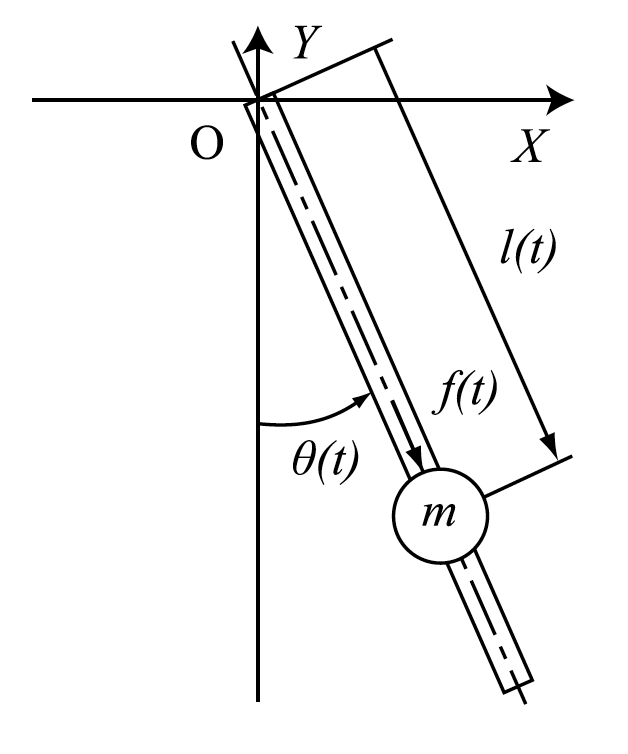
\includegraphics[width=0.96\textwidth,right]{images/vlp.png}
        \end{figure}
    \end{columns}
  \end{frame}

  \begin{frame}{Problem Formulation}
    Let $m=1$. Total mechanical energy:
    \begin{equation*}
      E_T = %T+P =
        \frac{1}{2}\dot{l}^2(t)+\frac{1}{2}\big(l(t)\dot{\theta}(t)\big)^2-
        gl(t)\cos\theta(t) 
    \end{equation*}
    Desired trajectory of swing described by:
    \begin{equation*}
      E_r = \frac{1}{2}\big(l_r\dot{\theta}(t)\big)^2-gl_r\cos\theta(t) 
    \end{equation*}
    with $E_r$ and $l_r$ desired energy and length of the VLP.\\Moreover:
    $E_r = -gl_r\cos\theta_{max}, \theta_{max} \in (0,\pi]$.

    \textbf{Trajectory tracking control problem:}
    \begin{equation*}
      \lim_{t\rightarrow \infty} E_T = E_r  \quad
      \lim_{t\rightarrow \infty} \dot{l} = 0 \quad
      \lim_{t\rightarrow \infty} l = l_r
    \end{equation*}
  \end{frame}

  \begin{frame}{Controller Design: Total Energy Shaping}
    Lyapunov candidate with $k_P>0$, $k_D>0$:
    \begin{gather*}
      V_c = \frac{1}{2}(E_T-E_r)^2+\frac{1}{2}k_P(l-l_r)^2+
        \frac{1}{2}k_D\dot{l}^2 \\
      \dot{V}_c = \dot{l}\big((E_T-E_r+k_D)u-(E_T-E_r)(l\dot{\theta}^2+
        g\cos\theta)-k_P(l-l_r) \big)
    \end{gather*}
    Controller:
    \begin{equation*}
      u = \frac{(E_T-E_r)(l\dot{\theta}^2+g\cos\theta)-k_P(l-l_r)-
        k_V\dot{l}}{E_T-E_r+k_D}
    \end{equation*}
    with $k_V>0$, then:
    \begin{equation*}
      \dot{V}_c = -k_V\dot{l}^2 \leq 0
    \end{equation*}
    which holds only if:
    \begin{equation*}
      E_T-E_r+k_D  \neq 0 \quad \forall t\geq 0
    \end{equation*}
  \end{frame}

  \begin{frame}{Controller Design: Total Energy Shaping}
    Consider the trajectory tracking control problem defined previously
    and $l_r=3\text{m}$, $\theta_{\max}=2\pi/5$, $g=9.81\text{m/s}^2$.
    Choosing $k_D=12$, $k_P=30$ and $k_V=12$ yields $l_{de}=1.42\text{m}$.
  \end{frame}

  \begin{frame}{Controller Design: Total Energy Shaping}
    \begin{figure}
      \caption{Time responses of $V$, $E_T-E_r$, $E_T-E_r+k_D$ and $u$
        with initial state
        $(\theta(0),l(0),\dot{\theta}(0),\dot{l}(0)) = (-\pi/6,2,0,0)$.}
      \vspace{-0.3cm}
      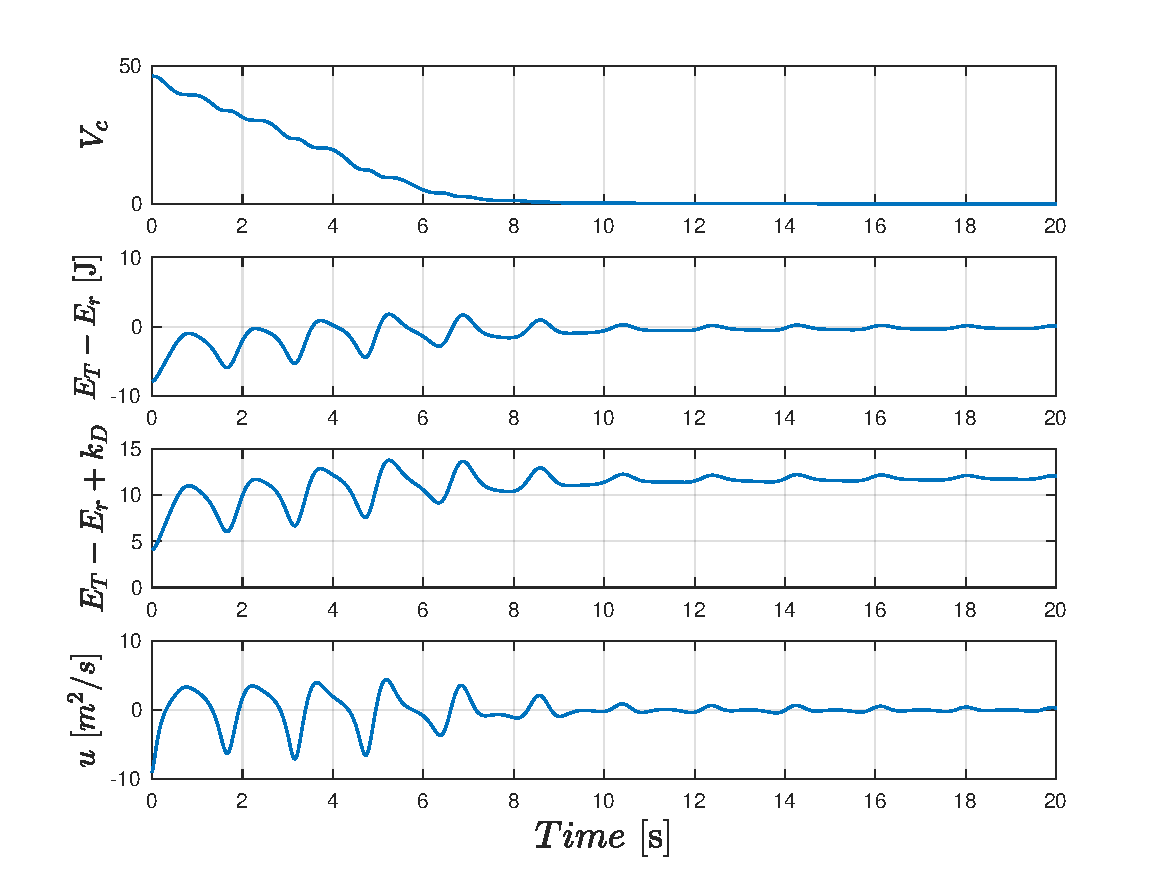
\includegraphics[width=0.8\textwidth]{images/total_1b.pdf}
    \end{figure}
  \end{frame}

  \begin{frame}{Controller Design: Total Energy Shaping}
    \begin{figure}
      \caption{Time reponses of $(\theta,l,\dot{\theta},\dot{l})$ with initial
        state $(\theta(0),l(0),\dot{\theta}(0),\dot{l}(0))=(-\pi/6,2,0,0)$.}
      \vspace{-0.3cm}
      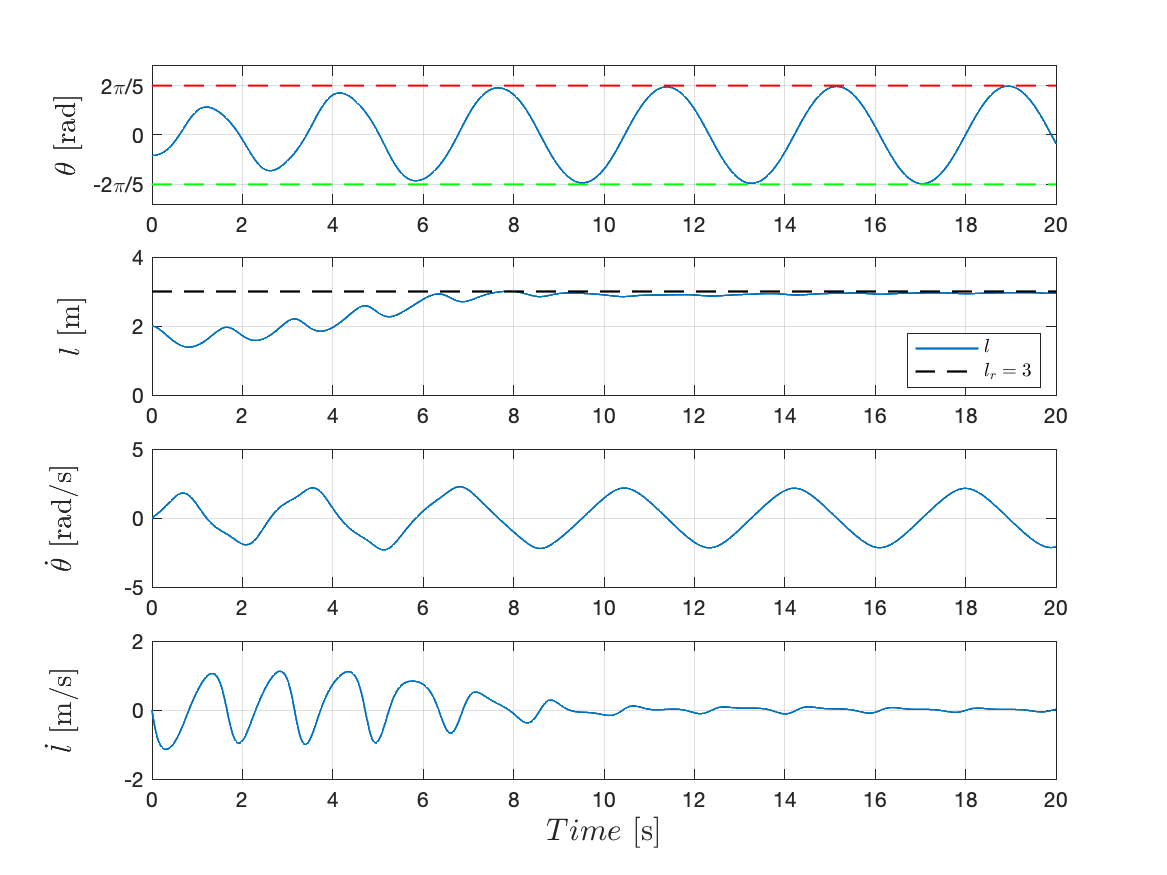
\includegraphics[width=0.8\textwidth]{images/total_2b.pdf}
    \end{figure}
  \end{frame}

  \begin{frame}{Controller Design: Total Energy Shaping}
    \begin{figure}
      \caption{The controller encountered a
        singular point for initial state $(\theta(0),l(0),\dot{\theta}(0),
        \dot{l}(0)) = (-\pi/6,2,0,4)$.}
      \vspace{-0.3cm}
      \begin{subfigure}{.49\textwidth}
        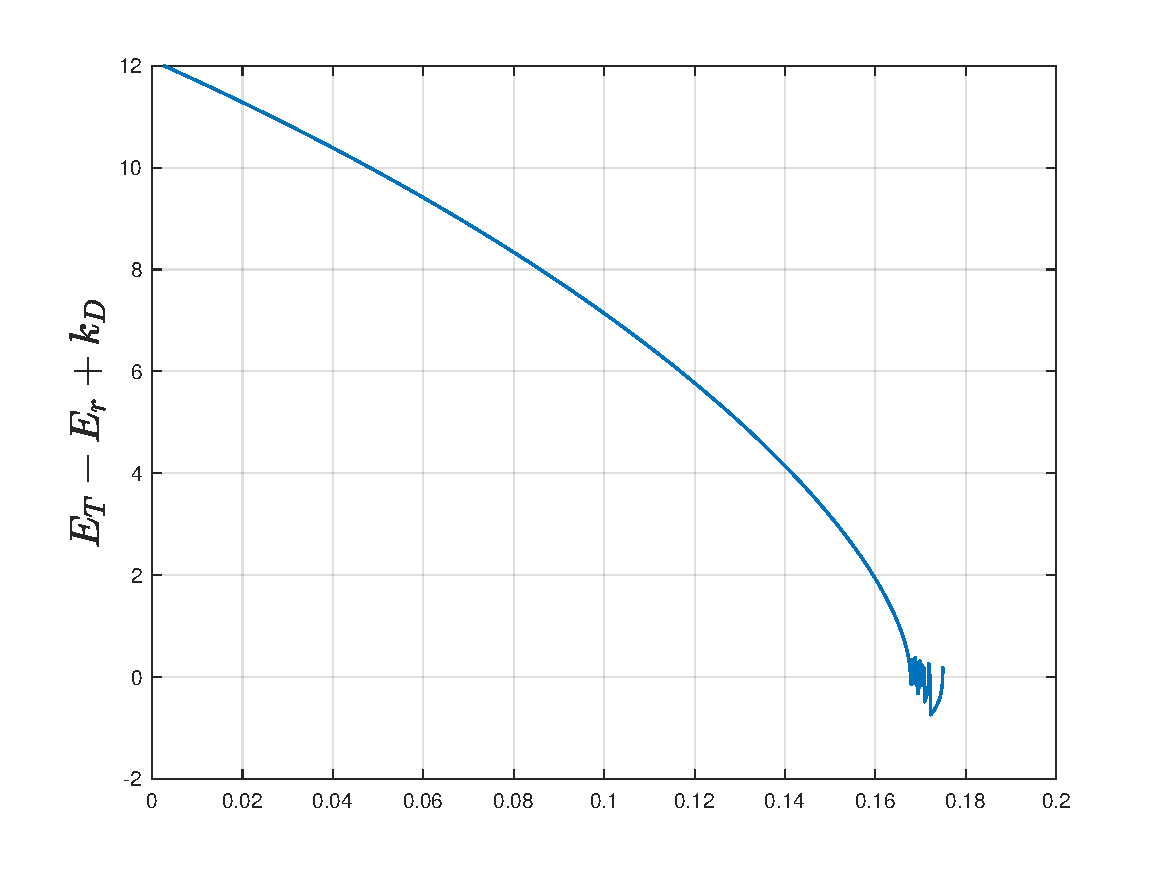
\includegraphics[width=1\linewidth]{images/total_2.pdf}
      \end{subfigure}
      \begin{subfigure}{.49\textwidth}
        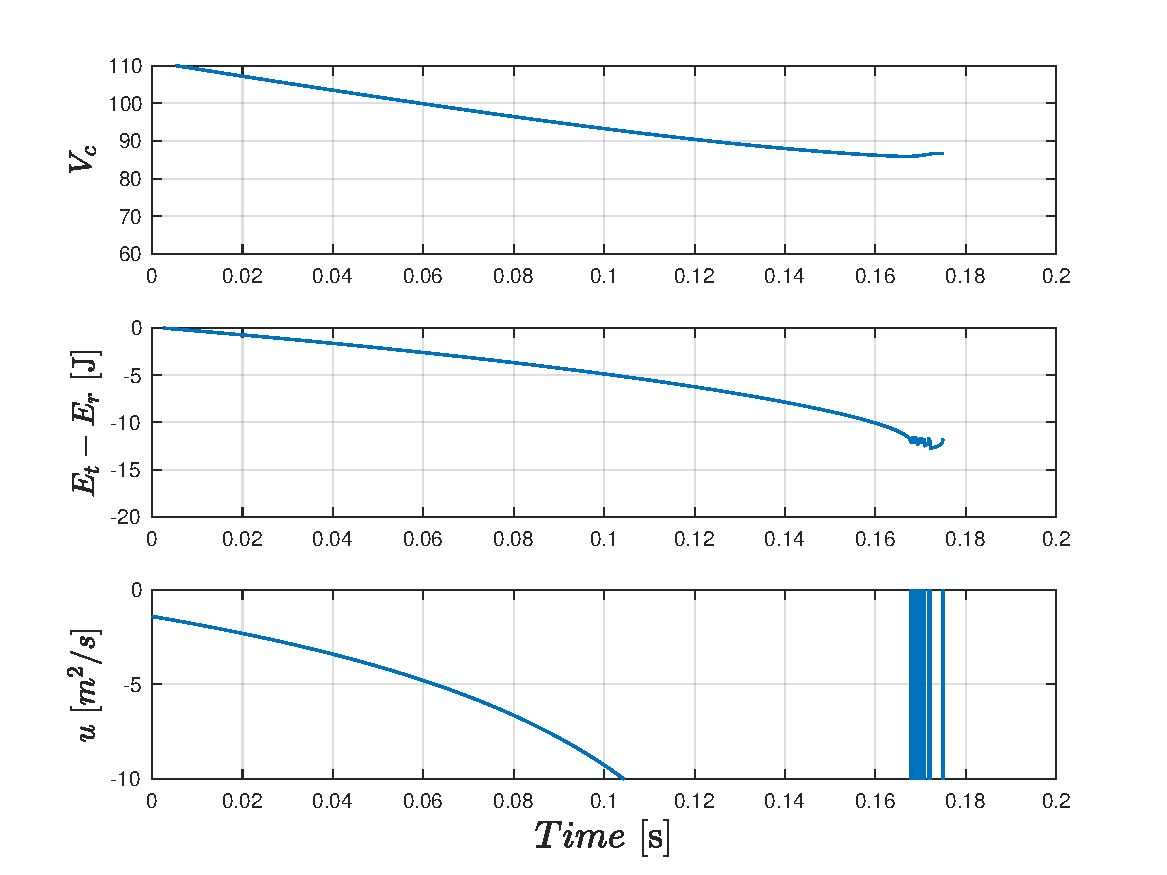
\includegraphics[width=1\linewidth]{images/total_1.pdf}
      \end{subfigure}  
    \end{figure}
  \end{frame}
  
  \begin{frame}{Controller Design: Partial Energy Shaping}
    $E_P$ sum of kinetic energy of rotation and potential energy of VLP:
    \begin{equation*}
      E_P = \frac{1}{2}(l(t)\dot{\theta}(t))^2-gl(t)\cos\theta(t)
    \end{equation*}
    Lyapunov candidate:
    \begin{gather*}
      V = \frac{1}{2}(E_P-E_r)^2+\frac{1}{2}k_P(l-l_r)^2+
        \frac{1}{2}k_D\dot{l}^2 \\ 
      \dot{V} = \big(-(E_P-E_r)(l\dot{\theta}^2+g\cos\theta)+k_P(l-l_r)\big)
        + k_D u) \dot{l}
    \end{gather*}
    Controller:
    \begin{equation*}
      u = \frac{(E_P-E_r)(l\dot{\theta}^2+g\cos\theta)-k_P(l-l_r)
        -k_V\dot{l}}{k_D}
    \end{equation*}
    which is free of singular points. Moreover:
    \begin{equation*}
      \dot{V} = -k_V \dot{l}^2 \le 0, \quad k_V > 0
    \end{equation*}
  \end{frame}

  \begin{frame}{Controller Design: Partial Energy Shaping}
    Consider:
    \begin{equation*}
      \Gamma_c = \left\{(\theta,l,\dot{\theta},\dot{l})|
        V(\theta,l,\dot{\theta},\dot{l}) \le c\right\}, \quad c > 0
    \end{equation*}
    Since $\dot{V} \le 0$, any closed-loop solution starting in $\Gamma_c$
    remains in $\Gamma_c$ for all $t \ge 0$.
    Let $W$ be the largest invariant set in:
    \begin{equation*}
      S = \{(\theta,l,\dot{\theta},\dot{l})) \in \Gamma_c|\dot{V}=0\}
    \end{equation*}
    Using \textbf{LaSalle's invariant principle}, every closed-loop
    solution starting in $\Gamma_c$ approaches $W$ as $t \to \infty$.
  \end{frame}

  \begin{frame}{Controller Design: Partial Energy Shaping}
    Since $\dot{V} = 0$ holds for all elements of $W$, $V$ and $l$
    are constant in $W$ (let them be $V^*$ and $l^*$). Moreover,
    since $V$ is a constant in $W$, $E_P$ is also a constant in $W$.
    Consequently:
    \begin{equation*}
      \lim_{t\rightarrow \infty} E_P = E^* \quad
      \lim_{t\rightarrow \infty} \dot{l} = 0 \quad
      \lim_{t\rightarrow \infty} l = l^*
    \end{equation*}     
    Thus, the largest invariant set $W$ can be defined as:
    \begin{equation*}
      W = \left\{(\theta,l,\dot{\theta},\dot{l})\middle|
        \frac{1}{2}(l^*\dot{\theta})^2-gl^*\cos\theta \equiv E^*,
        l \equiv l^*\right\}
    \end{equation*}
  \end{frame}

  \begin{frame}{Controller Design: Partial Energy Shaping}
    \begin{figure}
      \caption{Time responses of $V$, $E_P-E_r$ and $u$ with initial state 
        $(\theta(0), l(0), \dot{\theta}(0), \dot{l}(0))=(-\pi/6, 2, 0, 0).$}
      \vspace{-0.3cm}
      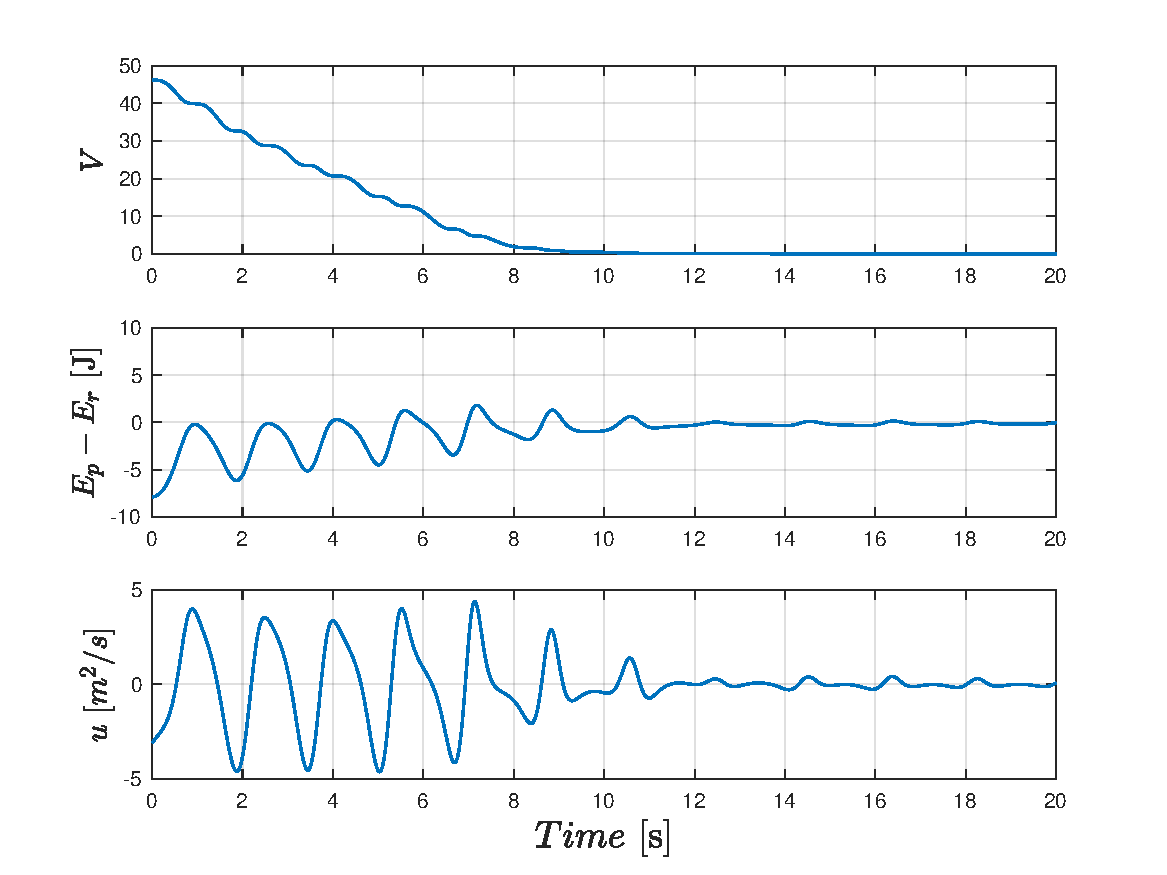
\includegraphics[width=0.8\textwidth]{images/partial_1.pdf}
    \end{figure}
  \end{frame}

  \begin{frame}{Controller Design: Partial Energy Shaping}
    \begin{figure}
      \caption{Time responses of $(\theta, l, \dot{\theta}, \dot{l})$ with 
        initial state $(\theta(0), l(0), \dot{\theta}(0), \dot{l}(0))=
        (-\pi/6, 2, 0, 0).$}
      \vspace{-0.3cm}
      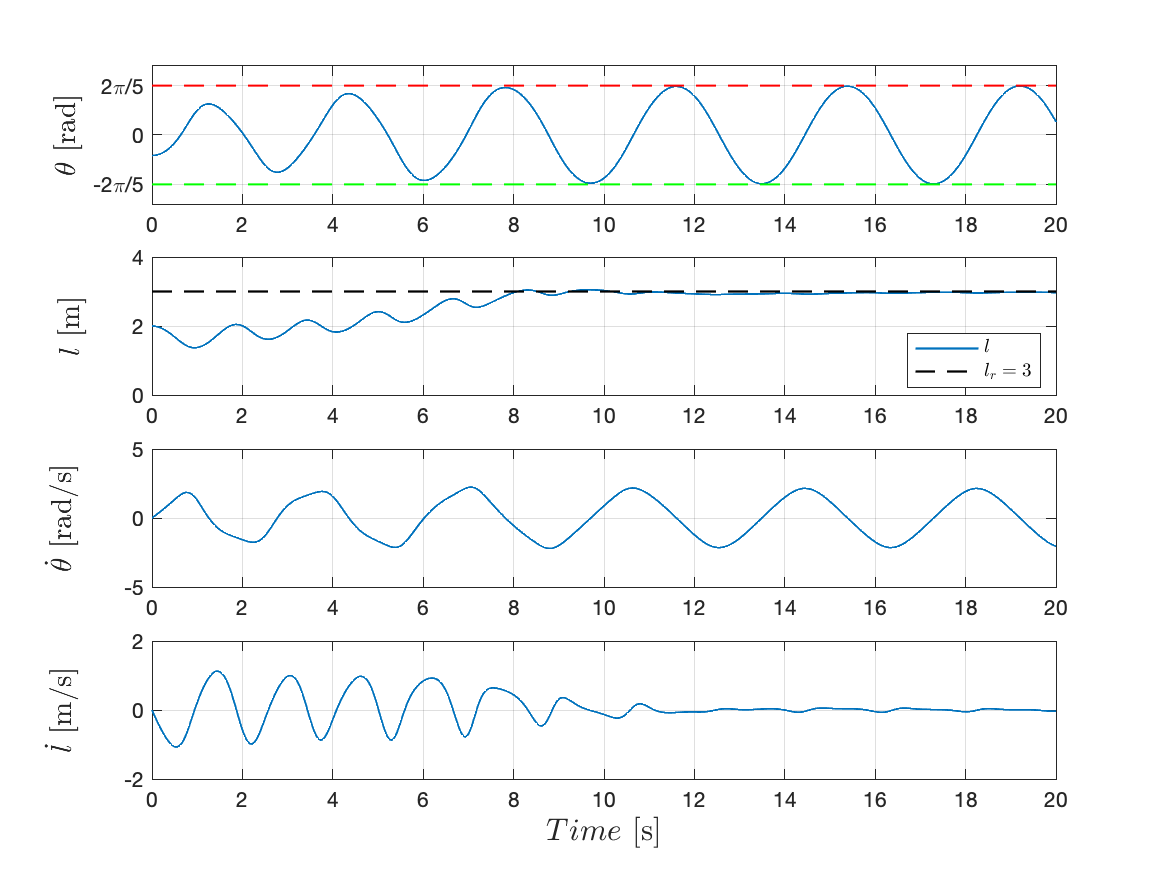
\includegraphics[width=0.8\textwidth]{images/partial_2.pdf}
    \end{figure}
  \end{frame}

  \begin{frame}{Controller Design: Partial Energy Shaping}
    \begin{figure}
      \caption{$V_\delta-V_{de}$.}
      \vspace{-0.3cm}
      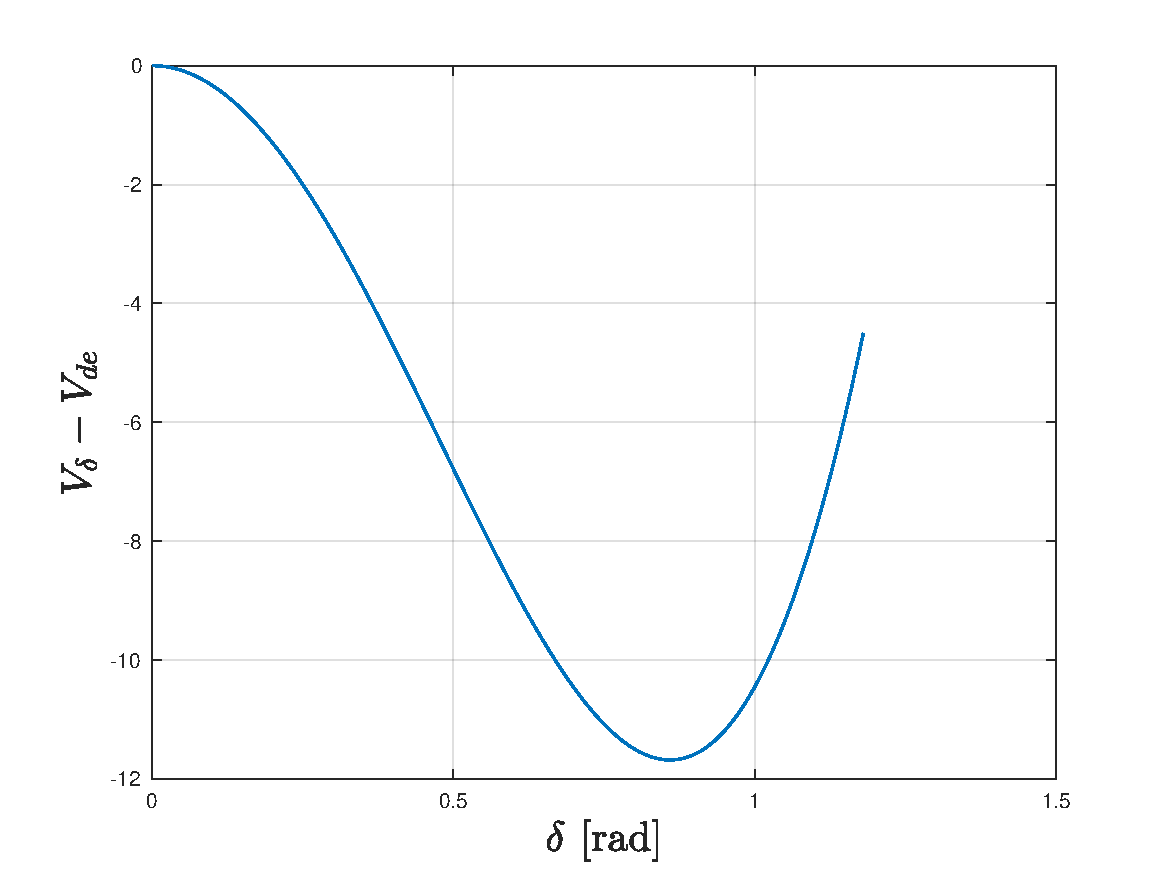
\includegraphics[width=0.8\textwidth]{images/partial_3.pdf}
    \end{figure}
  \end{frame}

  \begin{frame}{Motion Analysis: Convergence of Energy}
    Trajectory Tracking Control Problem achieved iff $V^*=0$, with:
    \begin{equation*}
      V^* = \frac{1}{2}(E^*-E_r)^2+\frac{1}{2}k_P(l^*-l_r)^2
    \end{equation*}
    Consider $E_P \equiv E^*$, $l \equiv l^*$, $\dot{l} \equiv 0$
    and $u = \ddot{l} \equiv 0$. Then, from the controller
    based on partial energy shaping:
    \begin{equation*}
      (E^*-E_r)(l^*\dot{\theta}^2+g\cos\theta)-k_P(l^*-l_r) \equiv 0
    \end{equation*}
  \end{frame}

  \begin{frame}{Motion Analysis: Convergence of Energy}
    \noindent \textbf{Case 1:} $E^* = E_r$

    In this case $l^* = l_r$. The largest invariant set $W$ becomes:
    \begin{equation*}
      W_r = \left\{ (\theta, l, \dot{\theta}, \dot{l})
        \middle| \frac{1}{2} (l_r \dot{\theta})^2 -
        g l_r \cos\theta \equiv E_r, l \equiv l_r \right\}
    \end{equation*}
    Hence, as $t \to \infty$, the closed-loop solution
    $(\theta(t), l(t), \dot{\theta}(t), \dot{l}(t))$ achieves the
    tracking control objective.
  \end{frame}

  \begin{frame}{Motion Analysis: Convergence of Energy}
    \noindent \textbf{Case 2} $E^* \neq E_r$

    In this case:
    \begin{equation*}
      l^* \dot{\theta}^2 + g\cos\theta \equiv \frac{k_P(l^*-l_r)}{E^*-E_r}
    \end{equation*}
    Considering $E_P \equiv E^*$ and $l \equiv l^*$ it is possible to prove
    that $\theta$ is a constant. Let $\theta \equiv \theta^*$. Moreover,
    since $E_r = -g l_r \cos\theta_{\max}$:
    \begin{equation*}
      l^* = \frac{l_r(k_P+g^2\cos\theta_{\max}\cos\theta^*)}{k_P+g^2}
    \end{equation*}
  \end{frame}

  \begin{frame}{Motion Analysis: Convergence of Energy}
    Since $\sin\theta^*=0$ admits a solution only in
    $\{0, \pi\}$, either $(\theta^*, l^*)=(\pi, l_{ue})$ or $(\theta^*,
    l^*)=(0, l_{de})$ where:
    \begin{align*}
      l_{ue} = l^*\rvert_{\theta^*=\pi} &=
        \frac{l_r(k_P-g^2\cos\theta_{\max})}{k_P+g^2} \\
        l_{de} = l^*\rvert_{\theta^*=0} &=
        \frac{l_r(k_P+g^2\cos\theta_{\max})}{k_P+g^2}
    \end{align*}
    To guarantee that the length
    of the pendulum $l_{ue}$ and $l_{de}$ are positive in the two
    cases respectively assume $k_P>-g^2\cos\theta_{\max}$ and
    $k_P>g^2\cos\theta_{\max}$, which can be rewritten as:
    \begin{equation*}
      k_P > g^2 |\cos\theta_{\max}|
    \end{equation*}
  \end{frame}

  \begin{frame}{Motion Analysis: Convergence of Energy}
    Considering also that $0 < \theta_{\max} \le \pi$,
    it is easy to prove that:
    \begin{gather*}
        0 < l_{ue} \le l_r \\ 0 < l_{de} < l_r
    \end{gather*}
    Let $\Omega$ be the equilibrium point set (which is an
    invariant set for the considered system) defined as follows:
    \begin{equation*}
      \Omega = \{ (\pi, l_{ue}, 0, 0), (0, l_{de}, 0, 0) \}
    \end{equation*}
  \end{frame}

  \begin{frame}{Motion Analysis: Closed-Loop Equilibrium Points}
    Consider the two equilibrium points defined in $\Omega$.
    Let the state variable vector be $x = (\theta, l, \dot{\theta},
    \dot{l})^T$. The state space representation is $\dot{x} = f(x)$,
    which, considering the dynamics of the VLP and the controller based on
    partial energy shaping, can be rewritten as: 
    \begin{align*}
      \dot{x}_1 &= x_3 \\
      \dot{x}_2 &= x_4 \\
      \dot{x}_3 &= -\frac{2 x_3 x_4 + g\sin x_1}{x_2} \\
      \dot{x}_4 &= \frac{(E_P-E_r)(x_2 x_3^2 + g\cos x1)
        -k_P(x_2-l_r)-k_V x_4}{k_D}
    \end{align*}
    where $E_P=x_2^2 x_3^2 / 2 - g x_2 \cos x_1$.
  \end{frame}

  \begin{frame}{Motion Analysis: Closed-Loop Equilibrium Points}
    The characteristic equation of the Jacobian matrix evaluated
    at the upper equilibrium point $x_{ue} = (\pi, l_{ue}, 0, 0)^T$
    yields:
    \begin{equation*}
      det(sI-A_{ue}) = \left( s^2 + \frac{k_V}{k_D}s +
        \frac{g^2+k_P}{k_D} \right) \left( s^2 - \frac{g}{l_{ue}}\right)
    \end{equation*}
    The jacobian $A_{ue}$ has three eigenvalues in the open LHP and
    one eigenvalue in the open RHP. Thus, the updward equilibrium point
    is unstable and \textbf{hyperbolic} (since all the eigenvalues of $A_{ue}$
    have non-zero real parts).
  \end{frame}

  \begin{frame}{Motion Analysis: Closed-Loop Equilibrium Points}
    The characteristic equation of the Jacobian matrix evaluated
    at the downward equilibrium point $x_{de} = (0, l_{de}, 0, 0)^T$ yields:
    \begin{equation*}
      det(sI-A_{de}) = \left( s^2 + \frac{k_V}{k_D}s +
        \frac{g^2+k_P}{k_D} \right) \left( s^2 + \frac{g}{l_{ue}}\right)
    \end{equation*}
    The Jacobian $A_{de}$ two eigenvalues in the open LHP and two
    eigenvalues on the imaginary axis.\\Thus, the downward equilibrium
    point is \textbf{non-hyperbolic} (since there
    is at least one eigenvalue on the imaginary axis).
  \end{frame}

  \begin{frame}{Motion Analysis: Closed-Loop Equilibrium Points}
    Consider the Lyapunov function V used for partial energy shaping:
    \begin{equation*}
      V = \frac{1}{2}(E_P-E_r)^2+\frac{1}{2}k_P(l-l_r)^2+
        \frac{1}{2}k_D\dot{l}^2
    \end{equation*}
    Consider the following set:
    \begin{equation*}
      \Gamma_d = \left\{ (\theta, l, \dot{\theta}, \dot{l})
        \mid V(\theta, l, \dot{\theta}, \dot{l}) <
        V(0, l_{de}, 0, 0) \right\}
    \end{equation*}
    Let the values of V at the downward equilibrium point $x_{de}$
    and a state $(\delta, l_{de}, 0, 0)$ be respectively $V_{de}$
    and $V_\delta$:
    \begin{gather*}
      V_{de} = V(0, l_{de}, 0, 0) = \frac{1}{2}(g l_{de} + E_r)^2
        + \frac{1}{2} k_P (l_{de} - l_r)^2 \\
      V_\delta = V(\delta, l_{de}, 0, 0) = \frac{1}{2}(g l_{de}
        \cos\delta + E_r)^2 + \frac{1}{2} k_P (l_{de} - l_r)^2
    \end{gather*}
  \end{frame}

  \begin{frame}{Motion Analysis: Closed-Loop Equilibrium Points}
    Compute the difference between $V_\delta$ and $V_{de}$ yields:
    \begin{align*}
      V_\delta - V_{de} %&= -\frac{1}{2} g l_{de} (1-\cos\delta)
        %(g l_{de}(1+\cos\delta)+2E_r) \\
        &= -\frac{g^2 l_{de} l_r (1-\cos\delta) \Xi}{k_P+g^2}
    \end{align*}
    where:
    \begin{equation*}
        \Xi = k_P(1-\cos\theta_{\max})-(k_P+g^2\cos\theta_{\max})
            \sin^2 \left( \frac{\delta}{2} \right)
    \end{equation*}
    Using $k_P > -g^2\cos\theta_{\max}$ and
    $|\sin \delta|<|\delta|$ for $\delta \neq 0$:
    \begin{equation*}
      \Xi > k_P(1-\cos\theta_{\max})-
        \frac{(k_P+g^2\cos\theta_{\max})\delta^2}{4}
    \end{equation*}
    with $\delta \neq 0$.
  \end{frame}

  \begin{frame}{Motion Analysis: Closed-Loop Equilibrium Points}
    If $\delta$ satisfies:
    \begin{equation*}
      0 < |\delta| \le \delta_m = 2
        \sqrt{\frac{k_P(1-\cos\theta_{\max})}{k_P+g^2\cos\theta_{\max}}}
    \end{equation*}
    then $\Xi>0$ (proof by simply noticing that $-\delta^2\ge-\delta_m^2$),
    which, using $V_\delta - V_{de}$, implies:
    \begin{equation*}
      V_\delta < V_{de}, \quad (\delta, l_{de}, 0, 0) \in \Gamma_d
    \end{equation*}
    which itself implies%, because of the definition of $\Gamma_d$,
    that $\Gamma_d \neq \varnothing$.
  \end{frame}

  \begin{frame}{Motion Analysis: Closed-Loop Equilibrium Points}
    Since $V$ is
    monotonically decreasing under the controller
    based on partial energy shaping, for any $\delta$
    satisfying $0 < |\delta| \le \delta_m$, closed-loop solution
    starting from $\Gamma_d$
    approaches $W_r$ due to the results obtained in
    Convergence of Energy (Case 1).
    Thus, the downward
    equilibrium point $(0, l_{de}, 0, 0)$ is unstable in the
    Lyapunov sense.

    Every closed-loop solution under the closed-loop
    system consisted of the dynamic equation of the VLP and the controller
    based on partial energy shaping, supposing
    $k_P>g^2|\cos\theta_{\max}|$, $k_D>0$, $k_V>0$,
    $0<\theta_{\max}\le\pi$, approaches $W=W_r\cup\Omega$.
  \end{frame}

  \begin{frame}{Controller Design: Partial Energy Shaping}
    \begin{figure}
      \caption{Time responses of $V$, $E_P-E_r$ and $u$ with initial state 
        $(\theta(0), \l(0), \dot{\theta}(0), \dot{l}(0))=(-\pi/3, l_{de}, 0,
        0)$, which satisfied $V_\delta < V_{de}$.}
      \vspace{-0.3cm}
      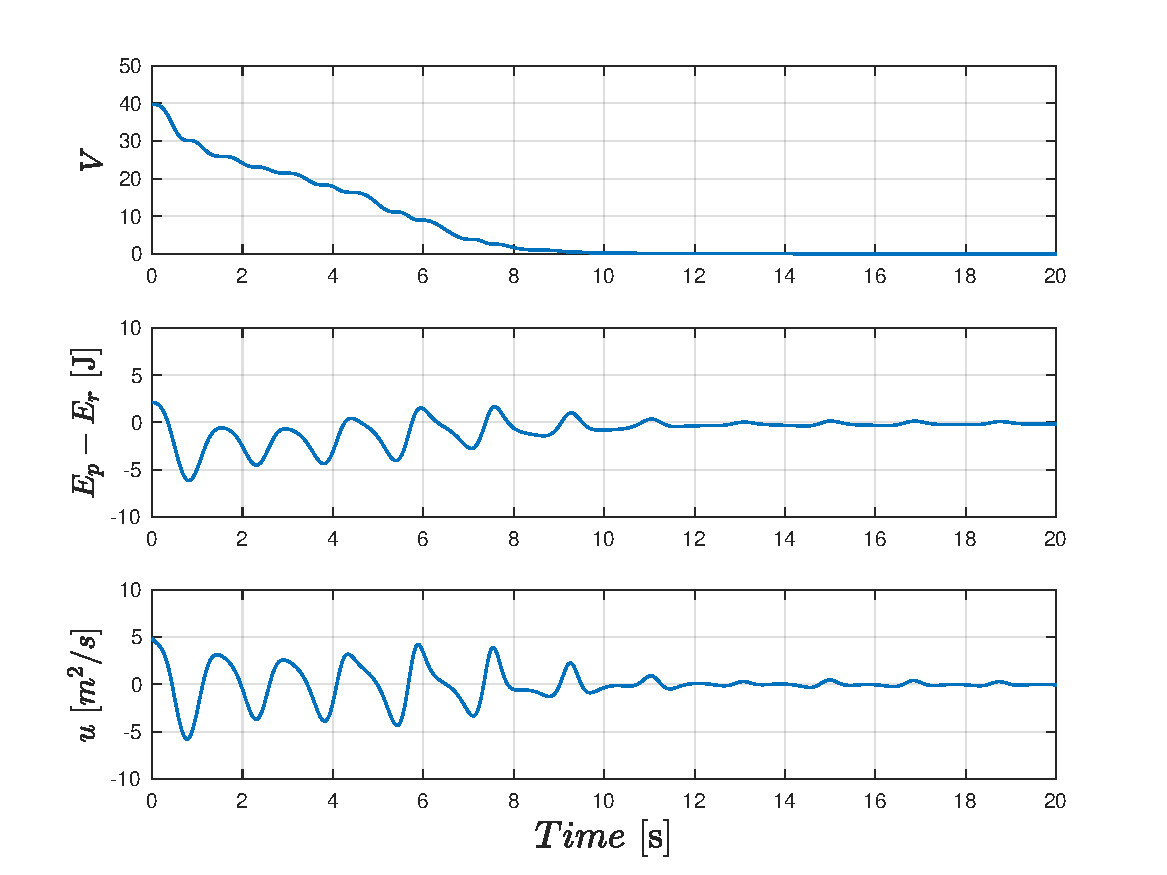
\includegraphics[width=0.8\textwidth]{images/partial_1b.pdf}
    \end{figure}
  \end{frame}

 \begin{frame}{Controller Design: Partial Energy Shaping}
    \begin{figure}
      \caption{Time responses of $(\theta, l, \dot{\theta}, \dot{l})$ with 
        initial state $(-\pi/3, l_{de}, 0, 0)$.}
      \vspace{-0.3cm}
      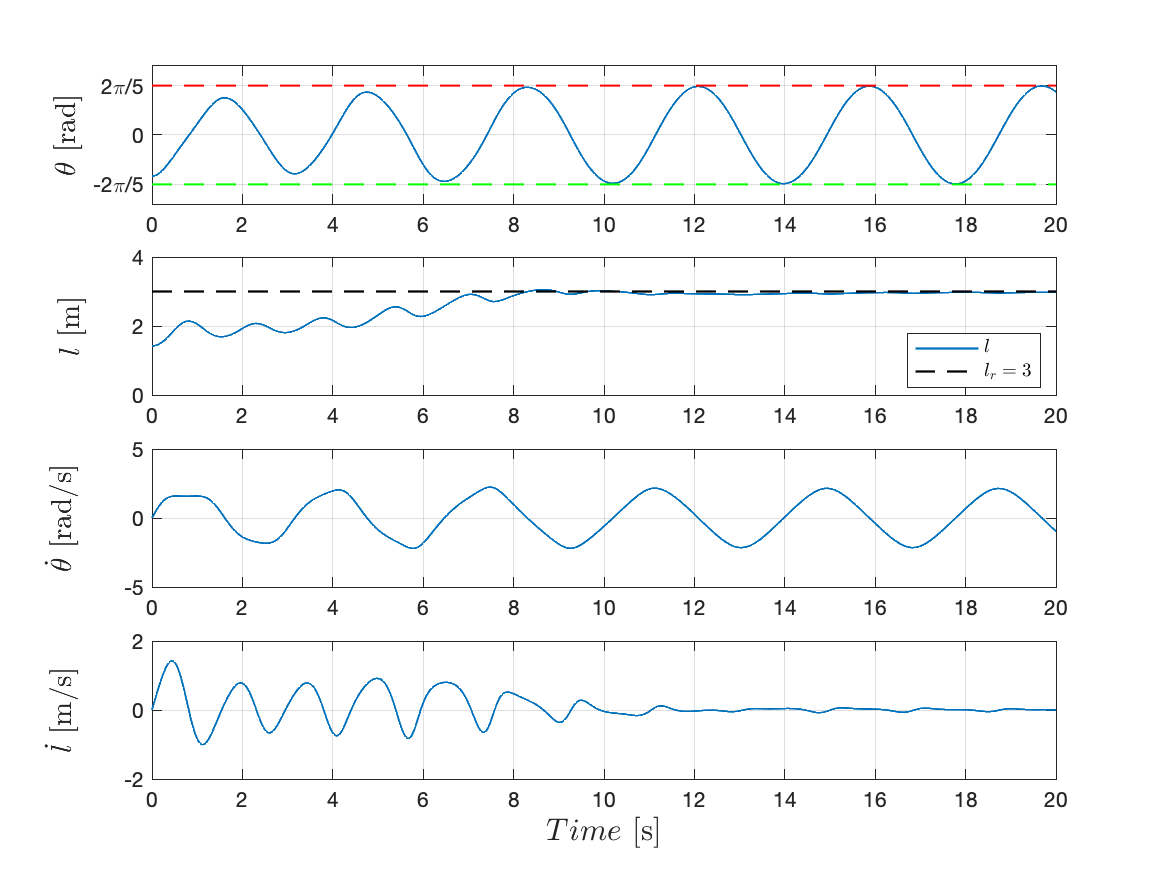
\includegraphics[width=0.8\textwidth]{images/partial_2b.pdf}
    \end{figure}
  \end{frame}

  \begin{frame}{Conclusion}
    \begin{itemize}
      \item Total Energy Shaping
      \item Partial Energy Shaping
      \item Motion Analysis
      \item Unstable Equilibrium Points
    \end{itemize}
  \end{frame}

  \begin{frame}[standout]
    Q\&A
  \end{frame}

  \appendix

  \begin{frame}{References}
    \bibliography{bibliography}
    \bibliographystyle{ieeetr}
  \end{frame}

\end{document}
